\section{Numerical Method}
\label{intro:numerical results in lower field}

As in the upper field, we will simulate a manufactured solution in order to verify the accuracy of our numerical scheme. We start by considering the basis function
$$v^w_p(x,z):=e^{i\tilde{p}x-i\gamma^w_pz},\quad \tilde{p}=\frac{2\pi p}{d},$$
where the phase $\exp(i \alpha x)$ is removed. We then utilize the exact Dirichlet/Neumann pairs $\{\zeta_r^w,\nu_r^w\}$ defined at the wavenumber $p=r$ and a profile $g(x)=\varepsilon f(x)$ where $\varepsilon > 0$ and our manufactured solutions are

\begin{subequations}
\begin{align}
\zeta_r^w(x)&:= B_r e^{i\tilde{r} x - i\gamma_r^w g(x)}, \\
\begin{split}
\nu_r^w(x) &:= [-\partial_z w_r + (\partial_x g)\partial_x w_r](x,g(x))\\&=
[(i\gamma_r^w)+\varepsilon(\partial_x f)(i\tilde{r})]B_r e^{i\tilde{r} x - i\gamma_r^w \varepsilon f(x)}.
\end{split}
\end{align}
\end{subequations}
To make the specification precise we solve, at every desired perturbation order $n$ and $m$, the elliptic boundary value problem, $(3.17)$,
%\vspace{-10mm}
\begin{subequations}
\begin{align}
\Delta w_{n,m} +2i\underline{\alpha}\partial_{x}w_{n,m}+(\underline{\gamma}^w)^2w_{n,m}&=\tilde{Y}_{n,m}\left(x,z;f,w,\underline{\alpha},\underline{\gamma}^w\right), &&\text{$-b<z<0$}, \\
w_{n,m}(x,0)&=\zeta^w_{n,m}(x),&& \text{at $z=0$},\\
w_{n,m}(x+d,z)&=w_{n,m}(x,z), \\
\partial_z \left[w_{n,m}(x,-b),\right] - T_0^w[w_{n,m}(x,-b)]&=\tilde{Q}_{n,m}(x),&& \text{at $z=-b$},
\end{align}
\end{subequations}
followed by the simulation of the $n$--th and $m$--th correction of the DNO, $(3.39)$,
\begin{equation*}J_{n,m}(f)[\zeta^w]=\partial_z w_{n,m}(x,0)- L_{n,m}(x;f,w).\end{equation*}
We begin by choosing the maximum perturbation orders, $N$ and $M$, and then approximate
\begin{equation}
w(x,z;\varepsilon,\delta)\approx w^{N,M}(x,z;\varepsilon,\delta):=\sum_{n=0}^N\sum_{m=0}^{M}w_{n,m}(x,z)\varepsilon^n\delta^m,
\end{equation}
\begin{equation}
J(x;\varepsilon,\delta)\approx J^{N,M}(x;\varepsilon,\delta) :=\sum_{n=0}^N\sum_{m=0}^{M}J_{n,m}(x)\varepsilon^n\delta^m,
\end{equation}
where, by the periodicity of solutions,
\begin{equation}w_{n,m}(x,z)=\sum_{p=-\infty}^{\infty}\hat{w}_{n,m,p}(z)e^{i\tilde{p} x},\quad J_{n,m}(x)=\sum_{p=-\infty}^{\infty}\hat{J}_{n,m,p}e^{i\tilde{p} x}.\end{equation}
Each of these $w_{n,m}(x,z)$ are then simulated by a 
Fourier--Chebyshev approach which posits the form
$$
w_{n,m}(x,z) \approx w_{n,m}^{N_x,N_z}(x,z)
  := \sum_{p = -N_x/2}^{N_x/2-1} \sum_{\ell=0}^{N_z}
  \hat{w}_{n,m,p,\ell} e^{i \tilde{p} x} 
  T_{\ell} \left( \frac{2z+b}{b} \right),
$$
where $T_{\ell}$ is the $\ell$--th Cheybshev polynomial.
The unknowns, $\hat{w}_{n,m,p,\ell}$ are recovered 
from $(3.45)$ by the collocation approach. As in $\S 2.11$, our HOPS/AWE algorithm requires $N_x \times N_z$ unknowns at every perturbation order $(n,m)$. We apply a Fourier spectral method in the lateral direction where we require $N_x$ equally--spaced gridpoints. In the vertical direction we use a Chebyshev spectral method where we choose $N_z + 1$ collocation points.
We then simulate the lower layer DNO from 
$(3.39)$, where the coefficients $J_{n,m}$ from $(3.48)$ are approximated by
$$
J_{n,m}(x) \approx J_{n,m}^{N_x}(x) 
  := \sum_{p=-N_x/2}^{N_x/2-1} \hat{J}_{n,m,p} e^{i \tilde{p} x},
$$
and the $\hat{J}_{n,m,p}$ are recovered from the
$\hat{w}_{n,m,p,\ell}$. Inserting the expansions $(3.48)$ into $(3.45)$ gives
\begin{subequations}
\begin{align}
\partial_z^2\hat{w}_{n,m,p}(z)+\left((\underline{\gamma}_p^w)^2-\tilde{p}^2-2\underline{\alpha}\tilde{p}\right)\hat{w}_{n,m,p}(z)&=\hat{\tilde{Y}}_{n,m,p}(z),&&\text{$-b<z<0$},\\
\hat{w}_{n,m,p}(0)&=\hat{\zeta}^w_{n,m,p},&& \text{at $z=0$},\\
\partial_z \left[\hat{w}_{n,m,p}(-b)\right] - \hat{T^w}[\hat{w}_{n,m,p}(-b)]&=\hat{\tilde{Q}}_{n,m,p},&& \text{at $z=-b$},
\end{align}
\end{subequations}
Through this, we can solve our two--point boundary value problem through our Chebyshev collocation method and we now turn to a  numerical implementation of our HOPS/AWE algorithm in Matlab. To begin, we approximate the lower layer Dirichlet and Neumann data through the expansions
$$\zeta_{\text{TFE}}^{N_x,N_z,N,M}=\sum_{n=0}^N\sum_{m=0}^M \zeta_{n,m}^{N_x,N_z}(x)\varepsilon^n\delta^m, \quad
\nu_{\text{TFE}}^{N_x,N_z,N,M}=\sum_{n=0}^N\sum_{m=0}^M \nu_{n,m}^{N_x,N_z}(x)\varepsilon^n\delta^m,$$
from which we can compute the relative errors
$$\text{Error} ~{\zeta^w_r}=\text{Error}_{\text{TFE}}(N_x,N_z,N,M):=\frac{\left|\zeta^w_r-\zeta_{TFE}^{Nx,Nz,N,M}\right|_{L^{\infty}}}{|\zeta^w_r|_{L^{\infty}}},$$
$$\text{Error}~{\nu^w_r}=\text{Error}_{\text{TFE}}(N_x,N_z,N,M):=\frac{\left|\nu^w_r-\nu_{TFE}^{Nx,Nz,N,M}\right|_{L^{\infty}}}{|\nu^w_r|_{L^{\infty}}}.$$

% NUMERICAL RESULTS
\begin{section}{Numerical Results}
For our first simulation we considered a profile with moderate interfacial and frequency perturbations and the following paramaters 
$$f(x)=e^{\cos(x)},\quad \alpha = 0, \quad \varepsilon = 10^{-4}, \quad \delta = 10^{-4}, \quad d=2\pi,\quad r=2,$$
$$B_r=-4.8,\quad \gamma^w = 1.15, \quad N_x = 32,\quad N_z=32, \quad N=M=4.$$
In Table III we report the results of our tests using both Padé and Taylor summation.
\vspace{2mm}
%\begin{table}[H]
\newpage
\label{First Numerical Tests Lower Layer}
\begin{longtable}[c]{llllll} \toprule
    {$N$} & {$M$} & {Error ${\zeta^w_r}$ (Taylor)} & {Error $\zeta^w_r$ (Padé)} & {Error $\nu^w_r$ (Taylor)} & {Error $\nu^w_r$ (Padé)}  \\ \midrule
0 & 2 & 0.000187563 & 0.000187563 & 8.47895e-05 & 8.47895e-05 \\
0 & 4 & 0.000187563 & 0.000187563 & 8.47895e-05 & 8.47895e-05 \\
1 & 2 & 0.000187563 & 0.000187563 & 8.47895e-05 & 8.47895e-05 \\
1 & 4 & 0.000187563 & 0.000187563 & 8.47895e-05 & 8.47895e-05 \\
2 & 2 & 5.4509e-08  & 5.02104e-09 & 2.65222e-08 & 4.42536e-09 \\
2 & 4 & 5.4509e-08  & 5.02104e-09 & 2.65222e-08 & 4.42536e-09 \\
3 & 2 & 5.4509e-08  & 5.02104e-09 & 2.65222e-08 & 4.42536e-09 \\
3 & 4 & 5.4509e-08  & 5.02104e-09 & 2.65222e-08 & 4.42536e-09 \\
4 & 2 & 5.4509e-08  & 5.02104e-09 & 2.65222e-08 & 4.42536e-09 \\
4 & 4 & 5.00595e-09 & 4.98285e-09 & 4.41455e-09 & 4.39911e-09 \\ \bottomrule
\\
\caption{Relative Error, Error ${\zeta^w_r}$ and Error $\nu^w_r$, versus perturbation orders $N$ and $M$, for the TFE approximations to the Dirichlet data, $\zeta^w_r$ $(3.44\text{a})$, and the Neumann data, $\nu^w_r$ $(3.44\text{b})$, where we used both Taylor Series and Padé approximants. Parameter choices are specified above where we investigated moderate boundary and frequency perturbations.}
\end{longtable}
%\vspace{1mm}
%\end{table}

\vspace{-2mm}
%\begin{flushleft}
As expected from spectral methods, our HOPS/AWE algorithm reaches reasonable accuracy at $N=M=4$ Taylor or Padé orders. We then simulated new results by increasing the number of Padé orders and decreasing the size of the interfacial and frequency perturbations. In Figure $10$, we considered $N=M=4,8,12,16$ Padé orders and plotted the Relative Error for $\zeta^w_r$ as we expanded up to $\varepsilon = 10^{-2},10^{-4},10^{-6},10^{-8}$ and $\delta = 10^{-2},10^{-4},10^{-6},10^{-8}$ simultaneously with Padé summation. In Figure $11$, we kept  $N=M=4$ Padé orders fixed and plotted the Relative Error for $\zeta^w_r$ as we expanded up to $\varepsilon= 10^{-2},10^{-4},10^{-6},10^{-8}$ and $\delta = 10^{-2},10^{-4},10^{-6},10^{-8}$ simultaneously with Padé summation.
%\end{flushleft}

\vspace{-19mm}
\begin{figure}[H]
\setcounter{figure}{10}
\centering
    \subfloat[Error ${\zeta^w_r}$ (Padé), $N=M=4$, $\varepsilon = \delta = 10^{-2}$]
    {{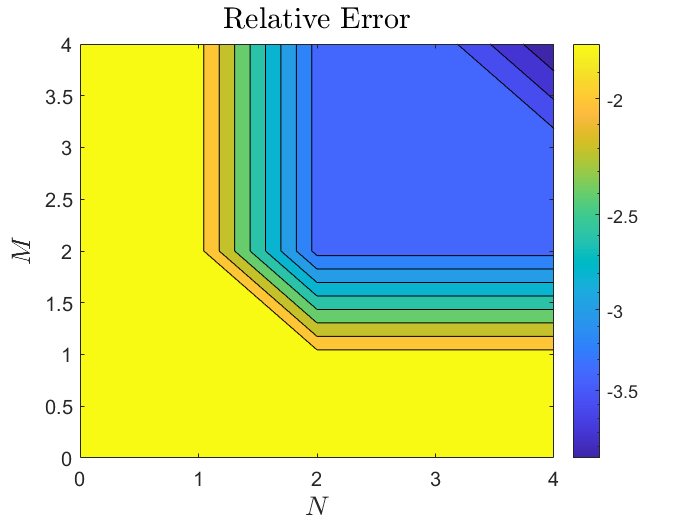
\includegraphics[width=7.6cm]{sections/3_lower_field/Error_Pade_Zeta_W_Intermediate_Profile_N_M_4_Eps_Delta_1e-2.png} }}
    \subfloat[Error ${\zeta^w_r}$ (Padé), $N=M=8$, $\varepsilon = \delta = 10^{-4}$]
    {{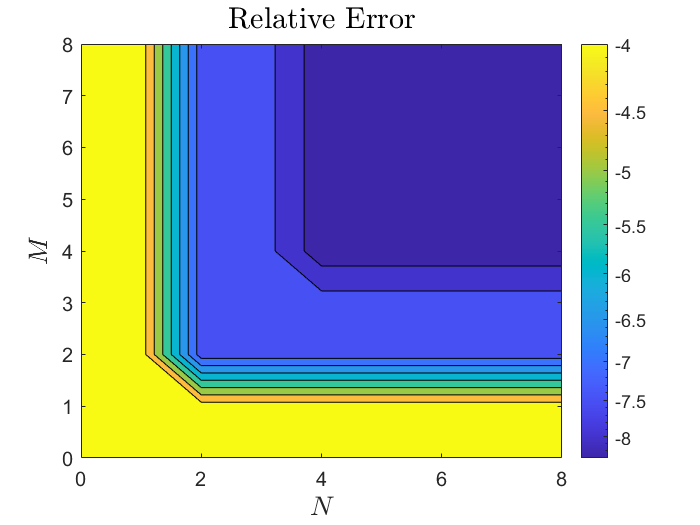
\includegraphics[width=7.6cm]{sections/3_lower_field/Error_Pade_Zeta_W_Intermediate_Profile_N_M_8_Eps_Delta_1e-4.png} }}
    \\
\end{figure}
\begin{figure}[ht]\ContinuedFloat
    \subfloat[Error ${\zeta^w_r}$ (Padé), $N=M=12$, $\varepsilon = \delta = 10^{-6}$]
    {{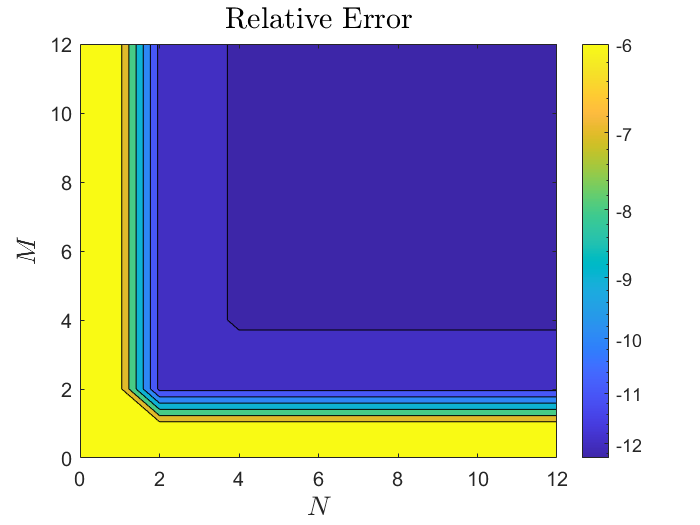
\includegraphics[width=7.6cm]{sections/3_lower_field/Error_Pade_Zeta_W_Intermediate_Profile_N_M_12_Eps_Delta_1e-6.png} }}
    \subfloat[Error ${\zeta^w_r}$ (Padé), $N=M=16$, $\varepsilon = \delta = 10^{-8}$]
    {{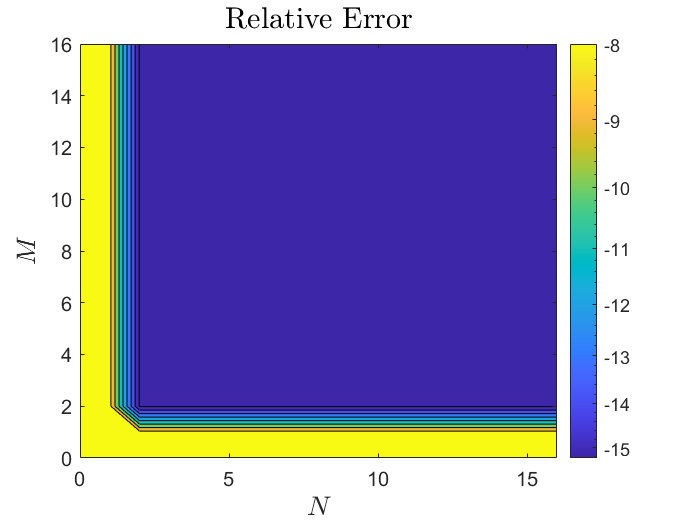
\includegraphics[width=7.6cm]{sections/3_lower_field/Error_Pade_Zeta_W_Intermediate_Profile_N_M_16_Eps_Delta_1e-8.png} }}
%\includegraphics[width=0.5\textwidth]{conv_N}
\vspace{3mm}
\caption{Plot of Relative Error for $\zeta^w_r$. Our HOPS/AWE algorithm used Padé summation with $N=M=4,8,12,16$ Padé orders to expand up to $\varepsilon = \delta = 10^{-2}, 10^{-4},10^{-6},$ $10^{-8}$ simultaneously. Physical parameters are reported in the profile above.}
%\label{Fig:N}
\end{figure}

\vspace{-41mm}
\begin{figure}[H]
\centering
    \subfloat[Error ${\zeta^w_r}$ (Padé), $\varepsilon = \delta = 10^{-2}$]
    {{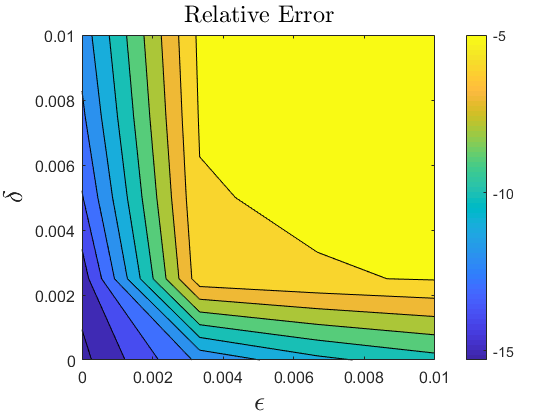
\includegraphics[width=7.6cm]{sections/3_lower_field/Error_Pade_Zeta_W_Intermediate_Profile_Eps_1e-2_Delta_1e-2.png} }}
    \subfloat[Error ${\zeta^w_r}$ (Padé), $\varepsilon = \delta = 10^{-4}$]
    {{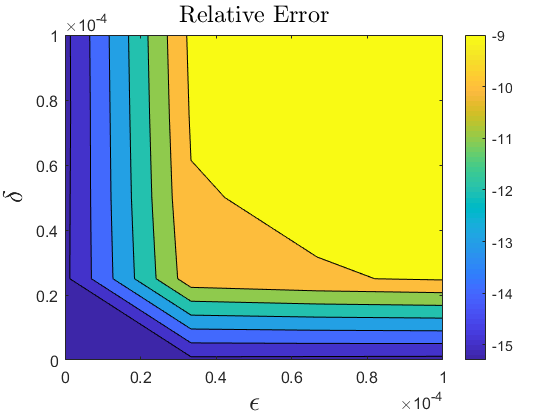
\includegraphics[width=7.6cm]{sections/3_lower_field/Error_Pade_Zeta_W_Intermediate_Profile_Eps_1e-4_Delta_1e-4.png} }}
    \\
    \subfloat[Error ${\zeta^w_r}$ (Padé), $\varepsilon = \delta = 10^{-6}$]
    {{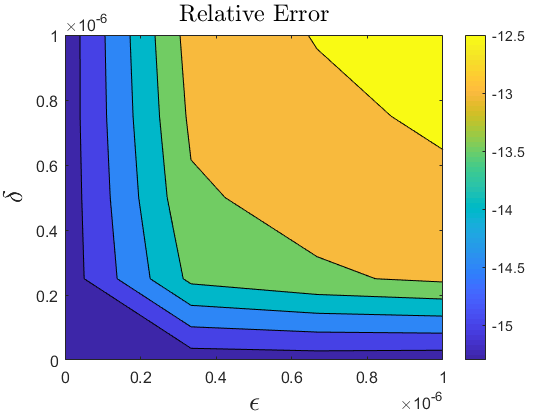
\includegraphics[width=7.6cm]{sections/3_lower_field/Error_Pade_Zeta_W_Intermediate_Profile_Eps_1e-6_Delta_1e-6.png} }}
    \subfloat[Error ${\zeta^w_r}$ (Padé), $\varepsilon = \delta = 10^{-8}$]
    {{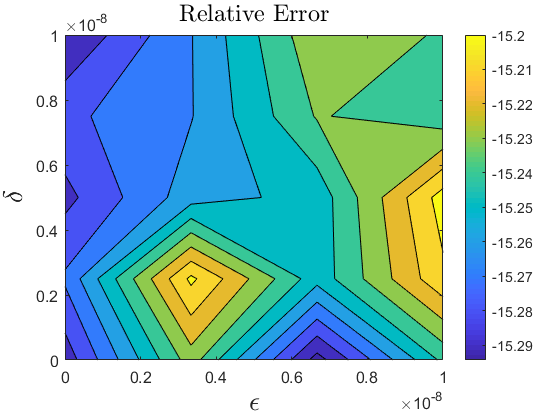
\includegraphics[width=7.6cm]{sections/3_lower_field/Error_Pade_Zeta_W_Intermediate_Profile_Eps_1e-8_Delta_1e-8.png} }}
%\end{figure}
%\includegraphics[width=0.5\textwidth]{conv_N}
%\vspace{3mm}
%\begin{figure}[ht]\ContinuedFloat
%\setcounter{figure}{10}
\vspace{3mm}
\caption{Plot of Relative Error for $\zeta^w_r$ with $N=M=4$ Padé orders fixed. Our HOPS/AWE algorithm used Padé summation to expand up to $\varepsilon = \delta = 10^{-2}, 10^{-4},10^{-6},10^{-8}$ simultaneously. Physical parameters are reported in the profile above.}
%\label{Fig:N}
\end{figure}
We then simulated an analytic profile with a smaller frequency perturbation and the following parameters
$$f(x)=\frac{1}{4}\sin(4x),\quad \alpha = 0, \quad \varepsilon = 10^{-4}, \quad \delta = 10^{-8}, \quad d=2\pi,\quad r=2,$$
$$B_r=-4.8,\quad \gamma^w = 1.15, \quad N_x = 32,\quad N_z=32, \quad N=M=4.$$
In Table IV we report the results of our tests using both Padé and Taylor summation.
\vspace{3mm}
%\begin{table}[H]
\label{Second Numerical Tests Lower Layer}
\begin{longtable}[c]{llllll} \toprule
    {$N$} & {$M$} & {Error ${\zeta^w_r}$ (Taylor)} & {Error $\zeta^w_r$ (Padé)} & {Error $\nu^w_r$ (Taylor)} & {Error $\nu^w_r$ (Padé)}  \\ \midrule
0 & 2 & 1.04998e-05 & 1.04998e-05 & 6.9068e-05  & 6.9068e-05  \\
0 & 4 & 1.04998e-05 & 1.04998e-05 & 6.9068e-05  & 6.9068e-05  \\
1 & 2 & 1.04998e-05 & 1.04998e-05 & 6.9068e-05  & 6.9068e-05  \\
1 & 4 & 1.04998e-05 & 1.04998e-05 & 6.9068e-05  & 6.9068e-05  \\
2 & 2 & 9.21284e-10 & 2.7964e-13  & 2.88241e-09 & 2.5317e-13  \\
2 & 4 & 9.21284e-10 & 2.7964e-13  & 2.88241e-09 & 2.5317e-13  \\
3 & 2 & 9.21284e-10 & 2.7964e-13  & 2.88241e-09 & 2.5317e-13  \\
3 & 4 & 9.21284e-10 & 2.7964e-13  & 2.88241e-09 & 2.5317e-13  \\
4 & 2 & 9.21284e-10 & 2.7964e-13  & 2.88241e-09 & 2.5317e-13  \\
4 & 4 & 8.25908e-14 & 9.3863e-14  & 3.1523e-13  & 2.50276e-13 \\ \bottomrule
\\
\caption{Relative Error, Error ${\zeta^w_r}$ and Error $\nu^w_r$, versus perturbation orders $N$ and $M$, for the TFE approximations to the Dirichlet data, $\zeta^w_r$ $(3.44\text{a})$, and the Neumann data, $\nu^w_r$ $(3.44\text{b})$, where we used both Taylor Series and Padé approximants. Parameter choices are specified by the analytic profile above.}
\end{longtable}
\vspace{-2mm}
\hspace{-6mm}In Figure 12, we kept  $N=M=4$ Taylor orders fixed and computed the Relative Error for $\nu^w_r$ as we expanded up to $\varepsilon= 10^{-2},10^{-4},10^{-6},10^{-8}$ and $\delta = 10^{-2},10^{-4},10^{-6},10^{-8}$ simultaneously. Jointly decreasing both perturbation variables simultaneously increased the accuracy of our HOPS/AWE algorithm and returned favorable convergence results for both $\varepsilon = \delta = 10^{-6}$ and $\varepsilon = \delta = 10^{-8}$.

\begin{figure}[H]
\centering
    \subfloat[Error ${\nu^w_r}$ (Taylor), $\varepsilon = \delta= 10^{-2}$]
    {{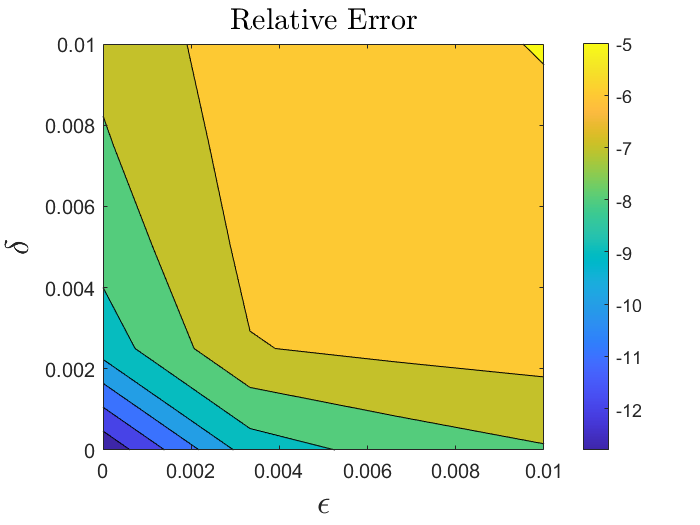
\includegraphics[width=7.6cm]{sections/3_lower_field/Error_Taylor_Nu_W_Good_Profile_Eps_1e-2_Delta_1e-2.png} }}
    \subfloat[Error ${\nu^w_r}$ (Taylor), $\varepsilon = \delta = 10^{-4}$]
    {{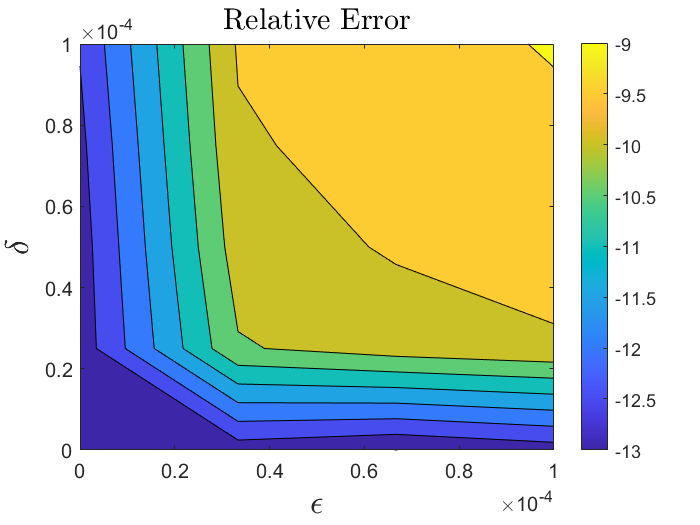
\includegraphics[width=7.6cm]{sections/3_lower_field/Error_Taylor_Nu_W_Good_Profile_Eps_1e-4_Delta_1e-4.png} }}
    \\
    %\end{figure}
    %\begin{figure}[ht]\ContinuedFloat
    \subfloat[Error ${\nu^w_r}$ (Taylor), $\varepsilon = \delta = 10^{-6}$]
    {{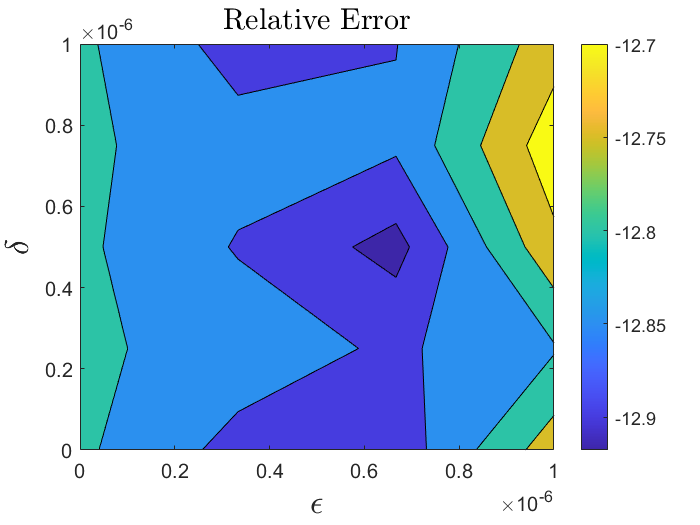
\includegraphics[width=7.6cm]{sections/3_lower_field/Error_Taylor_Nu_W_Good_Profile_Eps_1e-6_Delta_1e-6.png} }}
    \subfloat[Error ${\nu^w_r}$ (Taylor), $\varepsilon = \delta = 10^{-8}$]
    {{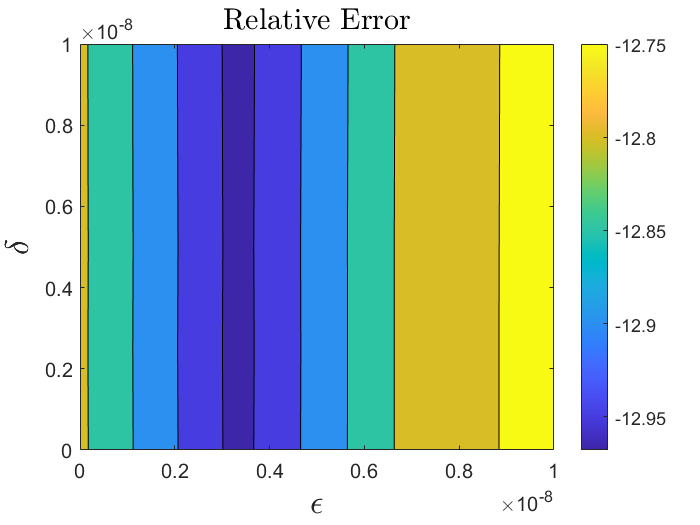
\includegraphics[width=7.6cm]{sections/3_lower_field/Error_Taylor_Nu_W_Good_Profile_Eps_1e-8_Delta_1e-8.png} }}
%\end{figure}
%\includegraphics[width=0.5\textwidth]{conv_N}
%\vspace{3mm}
%\begin{figure}[ht]\ContinuedFloat
\setcounter{figure}{11}
\vspace{3mm}
\caption{Plot of Relative Error for $\nu^w_r$ with $N=M=4$ Taylor orders fixed. Our HOPS/AWE algorithm used Taylor summation to expand up to $\varepsilon = 10^{-2}, 10^{-4},10^{-6},10^{-8}$ and $\delta = 10^{-2}, 10^{-4},10^{-6},10^{-8}$ simultaneously with the analytic profile above.}
%\label{Fig:N}
\end{figure}


